\section{Opgaver}

\begin{opgave}{Det Galileiske Relativitetsprincip}%fra 17
Det Galileiske Relativitetsprincip siger, at Newtons bevægelseslove er ens i alle inertielle referencesystemer.
Vi forestiller os nu et tog, der kører med en konstant hastighed $v$ ift. sporet. En passager i toget tager så en sten og slipper den fra hvile.
\opg Brug Galileis relativitetsprincip til at beskrive stenens bevægelse set fra en observatør i toget.
\opg Brug Galileitransformationerne \eqref{eq:galilei} til at give en beskrivelse af stenens bevægelse set fra en observatør på Jorden.
\end{opgave}

\begin{opgave}{Tog}%til galilei transformationen
En billetkontrollør går ned igennem et tog \SI{100}{m} langt tog.
\opg Hvis kontroløren går med en hastighed på $u=\SI{1}{\frac{m}{s}}$, hvor langt tid tager det kontroløren at gå fra bagenden til forenden af toget?\\\\
%
Toget kører med en hastighed på $v=\SI{20}{\frac{m}{s}}$ (\SI{72}{\frac{km}{h}}).
\opg  Brug Galileitransformationerne \eqref{eq:galilei} til at finde ud af hvor lang kontroløren har bevæget sig i forhold til omgivelserne.
(Hint: toget er $S'$)
\end{opgave}

\begin{opgave}{Kombination af Galileitranformationer}%fra 17
To tog kører parallelt med hinanden i $x$-retningen, det ene med hastighed $v$ og det andet med hastighed $u$, relativt til jorden. Lad det første tog være $S'$ og det andet $S''$, med deres respektive koordinater.
Jorden betegnes $S$.
\opg Hvad er Galileitransformationerne fra $S$ til $S''$?
\opg Hvad er Galileitransformationerne fra $S'$ til $S''$?
\opg Hvad svarer størrelsen $u-v$ til?
\end{opgave}

\begin{opgave}{Myoner i atmosfæren}
Når myoner bliver dannet i atmosfæren har de en hastighed 99\% af lysets hastighed.
Halveringstiden for en myon er \SI{1,5}{\mu s}.
\opg Hvad er halveringstiden for myonen for en observatør der står på Jordens overflade?
\opg Hvor langt når myonerne inden halvdelen af dem er henfaldet?
\opg Hvor stor en andel af de myoner der bliver dannet når jordoverfladen, når den bliver dannet i en højde af \SI{10}{km}?
\end{opgave}

\begin{opgave}{Pioner i atmosfæren}
Myoner er ikke de eneste partikler der bliver dannet af den kosmiske stråling.
Der bliver også dannet pioner, hvoraf de mest stabile, $\pi^+$ og $\pi^-$ har en halveringstid på \SI{18}{ns}.
De bliver også dannet med en hastighd på 99\% af lysets hastighed.
\opg Hvad er halveringtiden set fra jorden?
\opg Hvad er halveringslængden?
\opg hvor stor en andel af pionerne når jordoverfladen?
\opg Forventer du at man kan dedektere pioner fra den kosmiske stråling på jordoverfladen?
\end{opgave}

\begin{opgave}{Relativistisk Usain Bolt}
\SI{100}{m}-løberen Usain bolt, der har verdensrekorden, har en topfart på \SI{12,4}{\frac{m}{s}}
\opg Hvor langt ser de \SI{100}{m} ud når han løber med denne hastighed?
\opg Verdensrekorden i \SI{100}{m}-løb er \SI{9,572}{s}, hvor lang tid er det når man bevæger sig med Usain Bolts topfart?
\opg Hvad hvis lysets hastighed var \SI{15}{\frac{m}{s}}, hvor lang bliver \SI{100}{m} banen så?
\end{opgave}

\begin{opgave}{Myonens rejse}
En myon dannes i en højde af \SI{10}{km} med en hastighed på $0.99 c$.
\opg Set fra myonen, hvor langt ned er der?
\opg Med en halveringstid på \SI{1.5}{\mu s}, hvad er sandsyneligheden for at myonen når jordoverfladen?
\end{opgave}



\begin{opgave}{Lorentztransformation af forskelle}\label{opg:forskel}
Lad os se på to begivenheder $P_1$ og $P_2$, som i inertialsystemet $S$ har $(t_1,x_1)$  og $(t_2,x_2)$. Forskellen i de forskellige koordinater er
$$
\Delta t=t_2-t_1 \: ,~~~~\Delta x=x_2-x_1
$$\opg Find de tilsvarende forskelle $\Delta t'$ og $\Delta x'$ i $S'$.
\opg Hvad er transformationerne for koordinatforskelle?
\end{opgave}

\begin{opgave}{Tidsforlængelse og længdeforkortelse i Lorentztransformationerne}
Vi vil her vise at tidsforlængelse og længdeforkortning er specialtilfælde af Lorentztransformationerne.
Det gøres ved at se på en process set fra to referencesystemer $S$ og $S'$, hvor $S'$ bevæger sig langs $x$-aksen med hastighed $v$. starten og slutningen er adskildt rummeligt med $\Delta x$ og tidsligt $\Delta t $  i $S$. Tilsvarende er de adskildt med $\Delta x'$ og $\Delta t'$ i $S'$.
$\Delta x$ og $\Delta t$ transformerer som i opgave \ref{opg:forskel}
\opg Hvad skal vi kræve af $\Delta x$ og $\Delta t$, for at få udtrykket for tidsforlængelse?
\opg Hvad skal vi kræve af $\Delta x$ og $\Delta t$ for at få udtrykket for længdeforkortning?
\opg Hvad siger kravene til $\Delta x$ og $\Delta t$ om de underliggende $x_1$, $x_2$, $t_1$ og $t_2$?
\end{opgave}



\begin{opgave}{Tjek af Lorentztransformationerne}
Da vi udledte Lorentz så vi kun på de to første krav.
Her vil vi se på det 3. krav, at for små hastigheder vil Lorentztransformationerne være identisk med Galileitransformationerne.
En simpel tilnærmelse af en kompliceret funktion, er at finde en tangent, og bruge den i stedet.
\opg Find $\dv{\gamma}{v}$.
\opg Hvad er tangenten til $\gamma(v)$ omkring $v=0$?
\opg Hvad er Lorentztransformationerne under denne tilnærmelse.\\\\
%
Det vi her har set på kaldes en første ordens tilnærmelse.
Anden orden vil være
$$
\gamma(v)= \gamma(0)+\dv{\gamma}{v}(0)v+\frac{1}{2}\dv[2]{\gamma}{v}(0)v^2
$$
Her har vi en parabel, der i $v=0$ ikke bare har samme hældning, men også samme krumning.
\opg Hvad er anden ordens tilnærmelsen af Lorentztransformationerne?
\end{opgave}

\begin{opgave}{Addition af hastigheder}
Vi er vandt til, at man kan lægge hastigheder sammen. Så hvis vi har en kanon, der kan skyde et projektil afsted med en hastighed på $0,6c$, og vi placerer den på et tog, der også kan køre med $0,6c$, så ville det betyde, at set fra hvile ville vi så kunne sende projektilet afsted med en hastighed på $1,2c$. Det passer ikke med vores antagelser, så der er nok noget galt.\\
%
Vi ser på to inertialsystemer $S$ (jorden) og $S'$ (toget), der bevæger sig med en hastighed $v$.
\opg En person går med hastigheden $u$ i toget. Beskriv personens bevægelse i $S'$.
\opg Brug Galileitransformationerne til at beskrive bevægelsen af personen i toget set fra $S$.
\opg Brug istedet Lorentztransformationerne til at beskrive bevægelsen i $S$.
\opg Hvad sker der når både $v$ og $u$ er meget mindre end $c$?
\end{opgave}

\begin{opgave}{Jesus og Julius}
Cæsar blev myrdet i 44 f.Kr., og afstanden imellem Rom og Bethlehem er ca. \SI{2300}{km}.
\opg Findes der en iagttager, for hvilken Jesus' fødsel og Cæsars død var samtidige?
\opg Hvorfor/hvorfor ikke?
\end{opgave}

\begin{opgave}{Fulbert sover længe}%til rumtidsintervallet
Fulbert bor \SI{5}{km} fra skolen, og har sat sit vækkeur så han er klar til at tage af sted klokken kvart i otte, når han skal møde klokken otte.
\opg Hvad er rumtidsintervallet $\Delta s^2$ imellem Fulbert er klar, og han skal møde?\\\\
%
Fulbert kan godt lide at sove længe, så de fleste dage tager han lidt ekstra tid under dynen, så han først er klar klokken otte.
\opg Hvad er rumtidsintervallet så?\\\\
%
Fulberts lærere er blevet trætte af, at han altid kommer for sent.
De har sagt at han ikke må sove så længe at det ikke er fysisk muligt for ham at være i skole til tiden.
Som den aspirerende fysiker han er, tolker Fulbert det som at han ikke må overskride lysets hastighed.
\opg Hvornår skal Fulbert senest være klar til at tage af sted, og hvor stort er rumtidsintervallet imellem at han tager af sted, og han skal være fremme?
\end{opgave}

\begin{opgave}{Fulbert på rumrejse}
Fulbert drager ud på en rumrejse imens Beatrice bliver tilbage på Jorden.
Fulbert rejser med $0,8 c$, og rejser til Alfa Centauri, \SI{4,4}{\lightyear} borte.
\opg Hvor lang er rejsen set fra Fulbert når han er i bevægelse?
\opg Hvor lang tid tager Fulberts rejse for ham?
\opg Hvor lang tid tager rejsen set fra Beatrice?
\opg Fulbert vender hjemad lige efter han er nået frem. Hvor lang tid har hele rejsen taget for Fulbert?
\opg Hvor lang tid har Beatrice måttet vente på Jorden?
\end{opgave}


\begin{opgave}{Lyskeglen} \label{opg:LyskeglenOpgave}
Vi betragter begivenhederne indtegnet på figur \ref{fig:LyskegleOpgave}, som viser lyskeglen for med begivenheden $O$ som nu og her.
\opg Hvilke begivenheder kan ske på samme sted som begivenhed $O$, hvis observatøren er i bevægelse?
\opg Hvilke begivenheder kan ske på samme tidspunkt som begivenhed $O$, hvis observatøren er i bevægelse?
\opg Tegn en lyskegle for begivenhed $C$.
\opg Gentag delopgave 1 og 2 for begivenheden $C$.
\end{opgave}

\begin{figure}[h!]
    \centering
    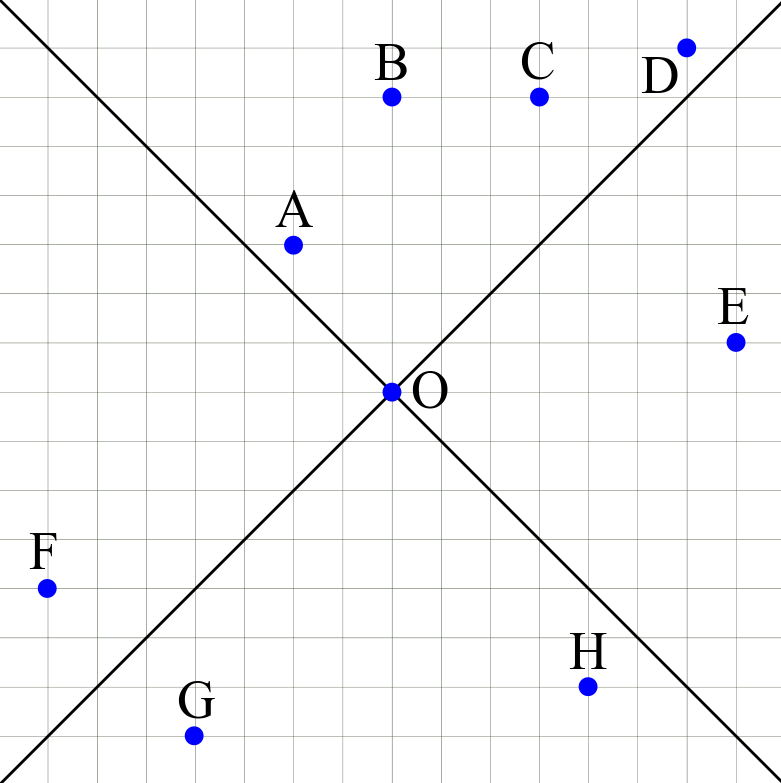
\includegraphics[width=0.5\textwidth]{opg/figurer/SR/Lyskegle.png}
    \caption{Lyskeglen fra opgave \thechapter,\ref{opg:LyskeglenOpgave} set med begivenhed $O$ som værende nu og her.}
    \label{fig:LyskegleOpgave}
\end{figure}